\documentclass[aps,prb,twocolumn,superscriptaddress,floatfix,longbibliography]{revtex4-2}



\usepackage[utf8]{inputenc}
\usepackage[spanish]{babel}
\usepackage{graphicx}
\usepackage{amsmath}
\usepackage{subcaption}
\usepackage{wrapfig} 
\usepackage[export]{adjustbox}

\usepackage{amsmath,amssymb} % math symbols
\usepackage{bm} % bold math font
\usepackage{graphicx} % for figures
\usepackage{comment} % allows block comments
\usepackage{textcomp} % This package is just to give the text quote '
%\usepackage{ulem} % allows strikeout text, e.g. \sout{text}

\usepackage[spanish]{babel}

\usepackage{enumitem}
\setlist{noitemsep,leftmargin=*,topsep=0pt,parsep=0pt}

\usepackage{xcolor} % \textcolor{red}{text} will be red for notes
\definecolor{lightgray}{gray}{0.6}
\definecolor{medgray}{gray}{0.4}

\usepackage{hyperref}
\hypersetup{
colorlinks=true,
urlcolor= blue,
citecolor=blue,
linkcolor= blue,
bookmarks=true,
bookmarksopen=false,
}

% Code to add paragraph numbers and titles
\newif\ifptitle
\newif\ifpnumber
\newcounter{para}
\newcommand\ptitle[1]{\par\refstepcounter{para}
{\ifpnumber{\noindent\textcolor{lightgray}{\textbf{\thepara}}\indent}\fi}
{\ifptitle{\textbf{[{#1}]}}\fi}}
\ptitletrue  % comment this line to hide paragraph titles
\pnumbertrue  % comment this line to hide paragraph numbers

% minimum font size for figures
\newcommand{\minfont}{6}

% Uncomment this line if you prefer your vectors to appear as bold letters.
% By default they will appear with arrows over them.
% \renewcommand{\vec}[1]{\bm{#1}}

%Cambiar Cuadros por Tablas y lista de...
%\renewcommand{\listtablename}{Índice de tablas}
\renewcommand{\tablename}{Tabla}
\renewcommand{\date}{Fecha}

\usepackage[bottom]{footmisc} %para que las notas al pie aparezcan en la misma página



\begin{comment}

%Comandos de interés:

* Para ordenar el documento:
\section{Introducción}
\section{\label{sec:Formatting}Formatting} %label para luego hacer referencia a esa sección

\ptitle{Start writing while you experiment} %pone nombre y título al documento dependiendo de si en el header están los comandos \ptitletrue y \pnumbertrue

* Ecuaciones:
\begin{equation}
a^2+b^2=c^2 \,.
\label{eqn:Pythagoras}
\end{equation}

* Conjunto de ecuaciones:
\begin{eqnarray}
\label{eqn:diagonal}
\nonumber d & = & \sqrt{a^2 + b^2 + c^2} \\
& = & \sqrt{3^2+4^2+12^2} = 13
\end{eqnarray}

* Para hacer items / enumerar:
\begin{enumerate}
  \item
\end{enumerate}

\begin{itemize}
  \item
\end{itemize}

* Figuras:
\begin{figure}[h]
    \includegraphics[clip=true,width=\columnwidth]{pixel-compare}
    \caption{}
     \label{fig:pixels}
\end{figure}

* Conjunto de figuras:
(no recuerdo)


* Para hacer referencias a fórmulas, tablas, secciones, ... dentro del documento:
\ref{tab:spacing}

* Para citar
Elementos de .bib
\cite{WhitesidesAdvMat2004}
url
\url{http://www.mendeley.com/}\\

* Agradecimientos:
\begin{acknowledgments}
We acknowledge advice from Jessie Zhang and Harry Pirie to produce Fig.\ \ref{fig:pixels}.
\end{acknowledgments}

* Apéndice:
\appendix
\section{\label{app:Mendeley}Mendeley}

* Bibliografía:
\bibliography{Hoffman-example-paper}

\end{comment}

\begin{comment}

Plots y tablas en orden:

* Figura de los cilindros con los PT100, la resistencia de referencia, la fuente, el multímetro y la computadora simbolizando el software de adquisisción de datos.
* Figura de los cilindros con la lampartira, la fuente que le da tensión y el multímetro para medir esa tensión

* Tabla de dimensiones de los cilindros
(la copio de prácticos anteriores)

* Figura del equipo de algto vacío (bomba mecánica, difusora, tubos, bridas, cámara, 3 cilindros...)
* Figura sobre cómo determinar epsilon (pirómetro, termocupla apoyados sobre cilindro exterior sin vacío)

PLOT PPAL:
* T vs t mostrando un gráfico lindo donde se vea bien el transitorio y el estacionario

SUBPLOTS:
* T vs t mostrando qué pasa si hay un cortocircuito interno que hace que la lámpara no prenda (se ven T bajas)
* T vs t mostrando qué pasa si no ponemos el telgopor
* T vs t mostrando qué pasa si falla el vacío
* T vs t mostrando qué pasa en el cilindro externo cuando agregamos N2
* T vs t mostrando qué pasa cuando cambiamos la potencia de la lamparita sobre la marcha



Determinación del producto de ctes
* T vs P recta para calcular la pendiente relacionada con el producto de constantes

Determinación de epsilon
* Gráfico Epsilon vs P

Bibliografía:
* Agregar referencia a la tabla de calibración R vs T
* Agregar referencia a que sacamos los datos de las áreas de un práctico de años anteriores

\end{comment}



\begin{document}

% Allows to rewrite the same title in the supplement
\newcommand{\mytitle}{Ejercicio 3 - TP 02 - Diferencias finitas - EDP }

\title{\mytitle}

\author{Pablo Chehade \\
    \small \textit{pablo.chehade@ib.edu.ar} \\
    \small \textit{Física computacional, Instituto Balseiro, CNEA-UNCuyo, Bariloche, Argentina} \\}


\maketitle

Se buscó resolver el siguiente sistema de ecuaciones no lineales

\begin{equation}
\frac{\partial u}{\partial t} = \mu \frac{\partial^2 u}{\partial x^2} + g_1(u,v)
\label{eq:edp_u}
\end{equation}

\begin{equation}
\frac{\partial v}{\partial t} = \nu \frac{\partial^2 v}{\partial x^2} + g_2(u,v)
\label{eq:edp_v}
\end{equation}

donde

\[ g_1(u,v) = \frac{1}{32} (-7 u^2 - 50 u v + 57) \]
\[ g_2(u,v) = \frac{1}{32} (7 u^2 + 50 u v  - 2 v - 55).\]

Las funciones $g_1$ y $g_2$ acoplan las evoluciones de $u$ y $v$, mientras que los coeficientes $\nu$ y $\mu$ condicionan la difusión del sistema.

Para resolver el problema se empleó un método numérico explícito de diferencias finitas en un dominio periódico discretizado con una grilla uniforme en el espacio y el tiempo. En particular, se empleó el método FTCS, asegurando la continuidad del flujo difusivo mediante la implementación de 'nodos fantasmas'. Se utilizaron condiciones iniciales al azar para ambas variables, con amplitud $0.15$ alrededor del equilibrio homogéneo $u^* = v^* = 1$, como se verifica en la figura \ref{fig:cond_inic}. Como coeficientes difusivos se emplearon $\mu = D$, $\nu = D/2$. La grilla uniforme tiene un tamaño total longitudinal $L = 1$, siendo $dx$ la unidad de la misma. Mientras que, temporalmente, tiene un tamaño total $t_{max}$ y unidad $dt$.

\begin{figure}[h]
    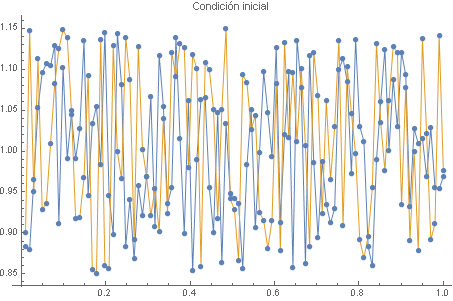
\includegraphics[clip=true,width=\columnwidth]{cond_inic}
    \caption{Condición inicial al azar. $u$ en color azul y $v$ en amarillo.}
     \label{fig:cond_inic}
\end{figure}

En primer lugar, se analizó la solución numérica bajo las condiciones $D = 0.01$, $dx = 0.01$ y $dt = 0.001$. Esta se representa para distintos tiempos en la figura \ref{fig:D_0.01}. Se observa que rápidamente la condición inicial cambia y evoluciona hacia una estructura periódica con longitud de onda $k = 2 \pi$ aproximadamente. Le toma al sistema alrededor de $t_{max} = 17.4 $ s para llegar al estado estacionario, momento en el que la solución deja de variar significativamente. Cabe aclarar que se determinó $t_{max}$ gráficamente; no se implementó un criterio cuantitativo. Además, se emplearon distintos tamaños de grilla $dx$ y $dt$ y se observó que para determinados valores la solución diverge. Esto se interpretó como un problema del método utilizado, no de la solución del sistema de EDP. En base a ello, en próximas experiencias se emplearon los valores $dx = 0.01$ y $dt = 0.001$.

\begin{figure}[h]
     \centering
     \begin{subfigure}[b]{0.3\textwidth}
         \centering
         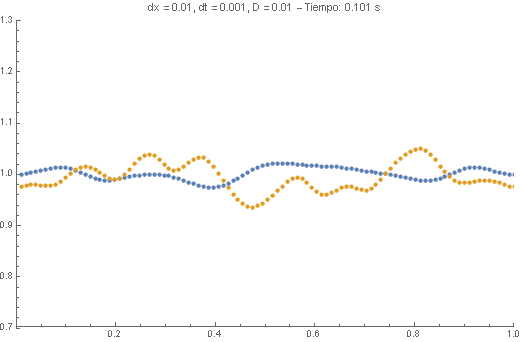
\includegraphics[width=\textwidth]{D_0.01_t1.png}
         \caption{\label{fig:D_0.01_t1}}
     \end{subfigure}
     \hfill
     \begin{subfigure}[b]{0.3\textwidth}
         \centering
         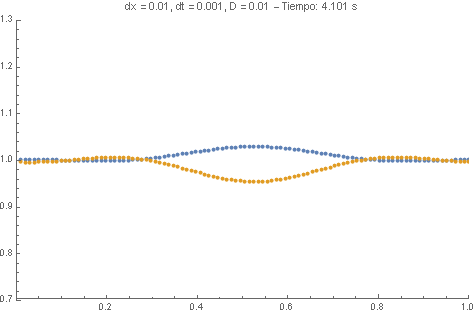
\includegraphics[width=\textwidth]{D_0.01_t2.png}
         \caption{\label{fig:D_0.01_t2}}
     \end{subfigure}
     \hfill
     \begin{subfigure}[b]{0.3\textwidth}
         \centering
         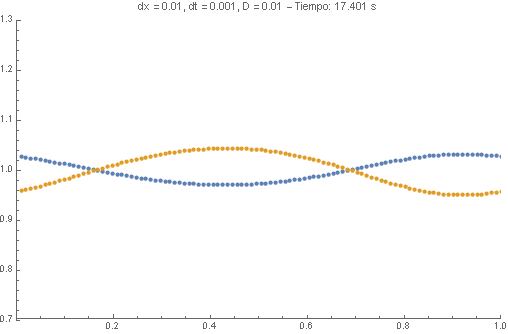
\includegraphics[width=\textwidth]{D_0.01_t3.png}
         \caption{\label{fig:D_0.01_t3}}
     \end{subfigure}
        \caption{Solución numérica para distintos tiempos bajo las condiciones $D = 0.01$, $dx = 0.01$ y $dt = 0.001$. $u$ en color azul y $v$ en color amarillo.}
        \label{fig:D_0.01}
\end{figure}

En segundo lugar, se analizó la influencia del factor $D$ en la solución numérica. Se consideraron los valores $D = 0.0025$, $0.001$, $0.0015$, $0.00075$. No se consideraron valores menores de $D$ debido ineficiencias del código y por no contar con suficientes recursos computacionales. Por ejemplo, el caso $D = 0.00075$ tomó más de una hora y media de ejecución. La solución inmediata sería aumentar $dx$ y $dt$ para que la grilla tenga menos puntos y la ejecución sea más rápida, pero no se encontraron valores tales que a tiempos grandes la solución no divergiera. Las soluciones en el estado estacionario se grafican en la figura \ref{fig:D_varios}. Se observa que el número de onda $k$ cambia dependiendo del parámetro $D$, siendo aproximadamente $4 \pi$ para $D = 0.0025$, $5 \pi$ para $D = 0.0015$ y $10 \pi$ para $D = 0.001$ y $D = 0.00075$. Realmente el número de onda para los últimos dos casos debería es distinto, pero dado que se midió $k$ gráficamente, el error asociado es grande y los valores se consideraron indistinguibles. Además, el parámetro $t_{max}$ aumenta a medida que disminuye $D$. Esto se debe a que la evolución es más lenta para coeficientes de difusividad menores.

\begin{figure}[h]
     \centering
     \begin{subfigure}[b]{0.3\textwidth}
         \centering
         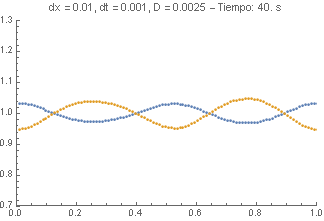
\includegraphics[width=\textwidth]{D_0.0025.png}
         \caption{\label{fig:D_0.0025}}
     \end{subfigure}
     \hfill
     \begin{subfigure}[b]{0.3\textwidth}
         \centering
         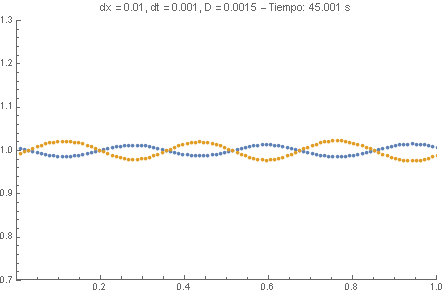
\includegraphics[width=\textwidth]{D_0.0015.png}
         \caption{\label{fig:D_0.0015}}
     \end{subfigure}
     \hfill
          \begin{subfigure}[b]{0.3\textwidth}
         \centering
         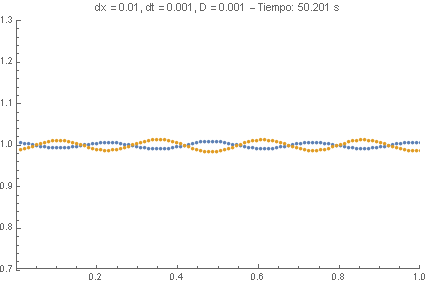
\includegraphics[width=\textwidth]{D_0.001.png}
         \caption{\label{fig:D_0.001}}
     \end{subfigure}
     \hfill
     \begin{subfigure}[b]{0.3\textwidth}
         \centering
         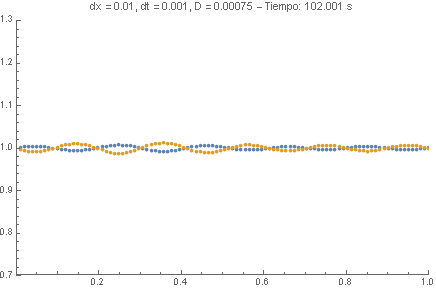
\includegraphics[width=\textwidth]{D_0.00075.png}
         \caption{\label{fig:D_0.00075}}
     \end{subfigure}
        \caption{Solución numérica para distintos valores de $D$ bajo las condiciones $dx = 0.01$ y $dt = 0.001$. $u$ en color azul y $v$ en color amarillo.}
        \label{fig:D_varios}
\end{figure}


\bibliography{Radiacion_de_cuerpo_negro}

\end{document}

